\chapter{Shape Prior}
\label{ch:shape-prior}

\begin{figure}
  \begin{subfigure}[t]{0.48\textwidth}
    \centering
    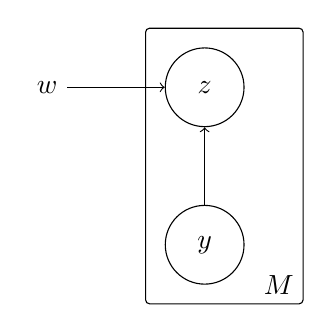
\begin{tikzpicture}

      \node[rectangle,rounded corners=0.05cm,draw=black,minimum width=2cm,minimum height=3.5cm] (M) at (0.25, -1){};
      \node[above left] at (M.south east){$M$};
      \node[circle,draw=black,minimum size=1cm] (z) at (0,0){$z$};
      \node[circle,draw=black,minimum size=1cm] (y) at (0,-2){$y$};
      \node[] (w) at (-2,0){$w$};
      
      \draw[->] (w) -- (z);
      \draw[->] (y) -- (z);
      
    \end{tikzpicture}
    \vskip 6px
    \caption{A graphical model illustration of the recognition model $q(z|y)$, \ie
    the encoder. Here, the parameters $w$ are used to model $q(z|y)$ using a neural network.}
    \label{subfig:shape-prior-encoder}
  \end{subfigure}\hfill
  \begin{subfigure}[t]{0.48\textwidth}
    \centering
    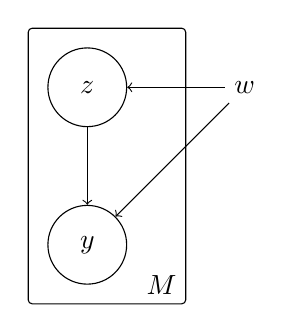
\begin{tikzpicture}

      \node[rectangle,rounded corners=0.05cm,draw=black,minimum width=2cm,minimum height=3.5cm] (M) at (0.25, -1){};
      \node[above left] at (M.south east){$M$};
      \node[circle,draw=black,minimum size=1cm] (z) at (0,0){$z$};
      \node[circle,draw=black,minimum size=1cm] (y) at (0,-2){$y$};
      \node[] (w) at (2,0){$w$};
      
      \draw[->] (w) -- (z);
      \draw[->] (w) -- (y);
      \draw[->] (z) -- (y);

    \end{tikzpicture}
    \vskip 6px
    \caption{An illustration of the generative model $p(y|z)$, \ie the decoder
    which is modeled using a neural network and parameters $w$.}
    \label{subfig:shape-prior-latent-decoder}
  \end{subfigure}
  \vskip 6px
  % TODO short caption
  \caption[]{Illustration of the graphical models corresponding to encoder and decoder,
  \ie recognition model $q(z|y)$ and generative model $p(y|z)$.}
  \label{fig:shape-prior}
\end{figure}

Given occupancy grids or signed distance functions of
the shape set $\mathcal{Y}$ and the observations $\mathcal{X}$,
our approach to Problem \ref{problem} involves two steps:
first, we learn a shape prior defining the space of allowed shapes;
and second, we learn an inference model to embed the observations
within the same latent shape space.
The shape prior defines a joint distribution $p(y, z) = p(y | z) p(z)$
of shapes $y$ and latent codes~$z$. Essentially, the shape prior
represents an embedding of the shapes $\mathcal{Y}$
within a low-dimensional latent space~$\mathcal{Z}$. By enforcing a 
prior $p(z)$ on the latent space, we are able to generate shapes
using $y \sim p(y|z)$ for $z \sim p(z)$. Additionally, shape completion
can be defined over the low-dimensional latent space by also learning
an embedding $x \mapsto z$ of observations $x$ within the latent space.
In our formulation of amortized maximum likelihood, this embedding is deterministic.
For the proposed extended variational auto-encoder, the embedding is also probabilistic,
\ie expressed as $q(z | x)$.

In the following, we intend to learn the shape prior
using variational auto-encoders on set of shapes $\mathcal{Y} = \{y_1, \ldots, y_M\}$.
For occupancy grids or signed distance functions, we assume a flattened version
$y \in \mathbb{R}^R \simeq \mathbb{R}^{H \times W \times D}$ for simplicity.
The latent space is then given as $\mathcal{Z} = \mathbb{R}^Q$ for 
small $Q \ll R$.
A variational auto-encoder is an implementation of the more general
continuous latent variable model, which can easily be summarized using
the two graphical models in Figure~\ref{fig:shape-prior}. Although we are
mainly interested in the generative model $p(y | z)$ given a fixed prior $p(z)$,
training also requires learning the recognition model $q(z | y)$
in order to maximize the overall likelihood $p(y)$. For simple Gaussian models,
the recognition model $q(z | y)$ as well as the so-called marginal likelihood
\begin{align}
  p(y) = \int p(y, z) dz = \int p(y | z)p(z) dz
  \label{eq:shape-prior-marginal-likelihood}
\end{align}
can usually be determined analytically,
\eg see the discussion of probabilistic principal component analysis in
Appendix \ref{ch:appendix-shape-prior}. In the case of variational auto-encoders,
both the generative and the recognition model are implemented using neural networks.
Then, the recognition model as well as the marginal likelihood can only be approximated
-- mainly because the integral in Equation \eqref{eq:shape-prior-marginal-likelihood}
becomes intractable. In this chapter, we first follow \cite{BleiKucukelbirMcAuliffe:2016}
and \cite{Doersch:2016}
to introduce the framework of variational inference which allows to maximize a
lower bound on the likelihood. Subsequently, we discuss two variants of variational
auto-encoders where the prior $p(z)$ is either modeled using Gaussian distributions
or based on Bernoulli distributions -- corresponding to continuous latent variables
or binary latent variables, respectively.

\section{Variational Inference}
\label{sec:variational-inference}

In general, variational inference is posed as the problem of
finding a model distribution $q(z)$ to approximate 
the true posterior $p(z | y)$
\begin{align}
  q(z) = \argmin_{q} \KL(q(z) | p(z | y))\label{eq:shape-prior-variational-inference}
\end{align}
where the Kullback-Leibler divergence $\KL$ is a distance measure defined
on probability distributions.
The Kullback-Leibler divergence can then be rewritten to obtain a
lower bound on the intractable marginal likelihood $p(y)$.
The Kullback-Leibler divergence is formally defined as
(see \cite[Section~A.1]{KollerFriedman:2009} or \cite[Section~1.6]{Bishop:2006}):

\begin{definition}
  The Kullback-Leibler divergence between two probability
  distributions $q(z)$ and $p(z|y)$ is defined as:
  \begin{align}
    \KL(q(z) | p(z|y)) = \mathbb{E}_{q(z)}\left[\ln\frac{q(z)}{p(z|y)}\right]
  \end{align}
  where $\mathbb{E}_{q(z)}$ denotes the expectation with respect to
  the distribution $q(z)$.
\end{definition}

%\begin{lemma}
%  For the Kullback-Leibler divergence as introduced above, it holds:
%  \begin{align}
%   \KL(q(z) | p(z|y)) \geq 0
%  \end{align}
%  and $\KL(q(z) | p(z|y))$ if and only if $q(z) = p(z|y)$ almost everywhere.
%\end{lemma}

%\begin{proof}
%  A proof can be found in \cite[Section~1.6]{Bishop:2006}.
%\end{proof}

% TODO formally introduce the expection value notation!
%Starting from the Kullback-Leibler divergence $\KL(q(z) | p(z|y))$ we follow
%\cite{BleiKucukelbirMcAuliffe:2016} to derive the evidence lower bound,
%a lower bound on the likelihood $p(y)$ to maximize as surrogate objective.
A close look at the Kullback-Leibler
divergence reveals that the optimization problem in Equation
\eqref{eq:shape-prior-variational-inference}
involves computing the marginal likelihood:
\begin{align}
  \KL(q(z) | p(z|y)) &= \mathbb{E}_{q(z)}\left[\ln\frac{q(z)}{p(z|y)}\right]\label{eq:shape-prior-variational-inference-kl}\\
   &= \mathbb{E}_{q(z)}[\ln q(z)] - \mathbb{E}_{q(z)}[\ln p(z|y)]\\
   &= \mathbb{E}_{q(z)}[\ln q(z)] - \mathbb{E}_{q(z)}[\ln p(z,y)] + \ln p(y).
\end{align}
Re-arranging left- and right-hand side leads to the evidence lower bound which is also
referred to as variational lower bound \cite{BleiKucukelbirMcAuliffe:2016}:
\begin{align}
  \ln p(y) &= \KL(q(z) | p(z|y)) - \mathbb{E}_{q(z)}[\ln q(z)] + \mathbb{E}_{q(z)}[\ln p(z,y)]\\
  &\geq - \mathbb{E}_{q(z)}[\ln q(z)] + \mathbb{E}_{q(z)}[\ln p(z,y)]\\
  &= - \mathbb{E}_{q(z)}[\ln q(z)] + \mathbb{E}_{q(z)}[\ln p(z)] + \mathbb{E}_{q(z)}[\ln p(y|z)]\\
  &= - \KL(q(z) | p(z)) + \mathbb{E}_{q(z)}[\ln p(y|z)]
\end{align}
The original problem of maximizing the intractable marginal likelihood $p(y)$ in Equation
\eqref{eq:shape-prior-marginal-likelihood} is then approximated
by maximizing the evidence lower bound which we formally define as:

\begin{definition}
  The variational lower bound or evidence lower bound derived from Problem
  \eqref{eq:shape-prior-variational-inference} is given by
  \begin{align}
    - \KL(q(z) | p(z)) + \mathbb{E}_{q(z)}[\ln p(y|z)]
    = \mathbb{E}_{q(z)}\left[\ln\frac{p(y, z)}{q(z)}\right]
    \label{eq:shape-prior-variational-lower-bound}
  \end{align}
\end{definition}

In this general formulation of the evidence lower bound, the model distribution
$q(z)$ can be arbitrary. However, in the context of latent variable models,
it makes sense to make the model distribution depend on $y$ explicitly, \ie $q(z | y)$,
as we want to be able to reconstruct any $y$ from the corresponding latent code $z$.
Then, the evidence lower bound in Equation \eqref{eq:shape-prior-variational-lower-bound}
takes the form of an auto-encoder where
$q(z | y)$ represents the encoder and $p(y | z)$ the decoder.
Thus, a variational auto-encoder can be trained by maximizing the right-hand-side
of Equation \eqref{eq:shape-prior-variational-lower-bound}
after choosing suitable parameterizations for the distributions $p(z)$ and $q(z | y)$.
In the following, we first discuss the Gaussian case.

\section{Gaussian Variational Auto-Encoder}
\label{sec:shape-prior-gaussian-vae}

% TODO distributions in figure
In the framework of variational auto-encoders
\cite{KingmaWelling:2013}, the model
distribution $q(z|y)$ is implemented as neural network; similarly,
$p(y|z)$ is modeled as neural network.
%As in
%Example \ref{ex:deep-learning-convolutional-auto-encoder},
%the recognition model $q(z|y)$ is referred to as encoder;
%the generative network $p(y|z)$ is referred to as decoder.
In the case of Gaussian variational auto-encoders,
both $q(z|x)$ and $p(z)$ are assumed to be Gaussian, specifically
\begin{align}
  q(z|y) &= \mathcal{N}(z; \mu(y;w), \diag(\sigma^2(y;w)))\label{eq:recognition-model}\\
  p(z) &= \mathcal{N}(z; 0, I_Q)\label{eq:prior-model}
\end{align}
where the dependence on the neural network weights $w$
is made explicit; \ie both the mean $\mu(y;w) \in \mathbb{R}^Q$
and the covariance matrix
$\diag(\sigma^2(y;w)) \in\mathbb{R}^{Q \times Q}$
are predicted using a neural network with parameters $w$ that
are to be optimized.In the following we will neglect the weights $w$
for brevity.

% TODO Monte Carlo sampling
Considering the evidence lower bound from Equation
\eqref{eq:shape-prior-variational-lower-bound}, \ie
\begin{align}
  \eqref{eq:shape-prior-variational-lower-bound}
  = - \KL(q(z|y)|p(z)) + \mathbb{E}_{q(z|y)}[\ln p(y|z)],
\end{align}
the Kullback-Leibler divergence between $q(z|y)$
and $p(z)$ can be computed analytically. However, differentiating the lower
bound with respect to the hidden weights in $q(z|y)$ is problematic.
A classical Monte-Carlo approximation of the expectation $\mathbb{E}_{q(z|y)}[\ln p(y|z)]$
would require differentiating through the sampling process $z \sim q(z | y)$.
Therefore, Kingma and Welling \cite{KingmaWelling:2013} proposed
the so-called reparameterization trick. In particular,
the random variable $z \sim q(z|y)$ is reparameterized using a
differentiable transformation $g(z, \epsilon)$ based on an auxiliary
variable $\epsilon$ drawn from a unit Gaussian:
\begin{align}
	z_i = g_i(y, \epsilon_i) = \mu_i(y) + \epsilon_i \sigma_i^2(y)
\end{align}
with $\epsilon_i \sim \mathcal{N}(\epsilon; 0, 1)$.
Overall, given a sample
$y_m \in \mathbb{R}^R$, the objective to be minimized has the form
\begin{align}
	\mathcal{L}_{\text{VAE}} (w) = \KL(q(z|y_m) | p(z))
	- \frac{1}{L}\sum_{l = 1}^L \ln p(y_m | z_{l,m})\label{eq:shape-prior-variational-auto-encoder-objective}
\end{align}
where $z_{l,m} = g(\epsilon_{l,m}, y)$ and $\epsilon_{l,m} \sim \mathcal{N}(\epsilon ; 0, I_Q)$.
Here, $L$ is the number of samples to use for the Monte Carlo estimator of the
reconstruction error. In practice, the loss $\mathcal{L}_{\text{VAE}}$ is applied on
mini-batches and $L = 1$ is usually sufficient.

% TODO VAEs as ``verification''
Given the neural network weights $w$, the generation process can be
summarized as follows: draw $z \sim p(z) = \mathcal{N}(z ; 0,I_Q)$,
and draw $y \sim p(y|z)$. Similarly, recognition is performed by
drawing $z \sim q(z|y)$, \ie $\epsilon \sim \mathcal{N}(\epsilon ; 0,I_Q)$
and $z = g(y,\epsilon)$. For evaluation purposes, \ie for
measuring the recognition performance, $z$ is usually set to
$z = \mathbb{E}_{q(z|y)}[z]$; this can be accomplished
by directly considering $\mu(y)$.

\subsection{Practical Considerations}

% TODO log to ln
% TODO always upper bound for sums and products
As mentioned above, the Kullback-Leibler divergence of two Gaussian
distributions can easily be calculated directly.
As we consider diagonal covariance matrices the Kullback-Leibler divergence
is separable over $1 \leq i \leq Q$. Then, following \cite[Section~9]{Kullback:1959} 
(also see \cite[Appendix~A]{RasmussenWilliams:2006}) we have
\begin{align}
  \KL(\mathcal{N}(z_i ; \mu_{1,i}, \sigma_{1,i}^2)|\mathcal{N}(z_i ; \mu_{2,i},\sigma_{2,i}^2))
  = \frac{1}{2} \ln\frac{\sigma_{2,i}}{\sigma_{1,i}} + \frac{\sigma_{1,i}^2}{2\sigma_{2,i}^2} + \frac{(\mu_{1,i} - \mu_{2,i})^2}{2 \sigma_{2,i}^2} - \frac{1}{2}.
\end{align}
and with $\sigma_{2,i} = 1$ and $\mu_{2,i} = 0$
(and for simplicity $\sigma_i^2 := \sigma_i^2(y) = \sigma_{1,i}^2$ and $\mu_i := \mu_i(y) = \mu_{1,i} $) it follows:
\begin{align}
  \KL(p(z_i | y) | p(z_i)) = - \frac{1}{2} \ln \sigma_i + \frac{1}{2} \sigma_i^2 + \frac{1}{2} \mu_i^2 - \frac{1}{2}.
  %&= \KL(\mathcal{N}(z_i ; \mu_i, \sigma_i^2) | \mathcal{N}(z_i ; 0, 1))\\
  \label{eq:shape-prior-analyitcal-kld}
\end{align}
%In practice, letting the encoder predict $\sigma^2(y)$ directly is problematic
%as $\sigma^2(y)$ may not be negative. We can avoid this constraint by predicting
%log-variances instead, \ie $l_i(y) := \ln \sigma_i^2(y)$. Then, the Kullback-Leibler
%divergence from Equation \eqref{eq:shape-prior-analyitcal-kld} changes to
%\begin{align}
%  \KL(\mathcal{N}(y_i ; y_i, l_i) | \mathcal{N}(y_i ; 0, 0))
%  = -\frac{1}{2}l_i + \frac{1}{2} \exp(l_i) + \frac{1}{2} \mu_i^2 - \frac{1}{2}
%\end{align}
%and the reparameterization trick can be written as
%\begin{align}
%  z_i = g(y, \epsilon_i) = \mu_i + \epsilon_i \exp\left(\frac{1}{2}l_i\right).
%\end{align}

% TODO losses parameters
The remaining part of the objective
is the reconstruction error, \ie the negative log-likelihood $- \ln p(y | z_l)$.
This depends on how $p(y|z)$ is modeled; in our case, $p(y|z)$
is decomposed element-wise over voxels:
\begin{align}
  p(y|z) = \prod_{i = 1}^R p(y_i | z)\quad\Rightarrow\quad -\ln p(y | z) = -\sum_{i = 1}^R \ln p(y_i | z)
\end{align}
For shapes $y$ in the form of occupancy grids, we use Bernoulli distributions
to model individual voxels, \ie $p(y_i | z) = \Ber(y_i ; \theta_i(z))$ where
the probabilities of occupancy $\theta_i(z)$ are predicted using the decoder.
The negative log-likelihood then 
reduces to the binary cross entropy error. When working with signed distance functions,
we use Gaussian distributions with fixed variance to model individual voxels,
\ie $p(y_i | z) = \mathcal{N}(y_i; \mu_i(z), \sigma^2)$ where the $\mu_i(z)$'s
are predicted by the decoder. In this case, the negative log-likelihood leads
to the sum-of-squared error. See Section \ref{sec:deep-learning-losses} for details.

For illustration and implementation purposes, we define two additional layers:

% TODO indicate Gaussian
\begin{definition}
  \label{def:shape-prior-kld-layer}
  A Gaussian Kullback-Leibler divergence layer $\text{KLD}_{\mathcal{N}}$
  takes as input two tensors $\mu \in \mathbb{R}^{B \times Q}$ and
  $\sigma^2 \in \mathbb{R}^{B \times Q}$ and computes the Kullback-Leibler
  divergence
  \begin{align}
    \sum_{b = 1}^B \KL(\mathcal{N}(z;\mu_b,\diag(\sigma_b^2)) | \mathcal{N}(z;0,I_Q)),
  \end{align}
  before passing the predicted $\mu_b, \sigma_b^2 \in \mathbb{R}^Q$
  on to the next layer (unchanged):
  \begin{align}
    \text{KLD}_{\mathcal{N}}(\mu, \sigma^2) = (\mu, \sigma^2).
  \end{align}
\end{definition}

% TODO write it exactly!
Essentially, this layer just makes the computation of the Kullback-Leibler
divergence explicit -- in a separate layer. This means that the forward pass
is unaffected. However, it is important to consider the derivatives
with respect to the predicted $\mu(y)$ and $\sigma^2(y)$ as these
need to be added to the decoder's gradients (coming from the reconstruction loss)
during error backpropagation in order to account for the Kullback-Leibler divergence
during training:
\begin{align}
  \frac{\partial \KL(p(z_i|y) | p(z_i))}{\partial \mu_i} = \mu_i
  \quad\text{ and }\quad
  \frac{\partial \KL(p(z_i|y) | p(z_i))}{\partial \sigma_i} = - \frac{1}{2\sigma_i} + \sigma_i
  %\quad\Leftrightarrow\quad \frac{\partial \KL(\mathcal{N}(y_i ; \sigma_i, l_i) | \mathcal{N}(y_i; 0, 0)}{\partial l_i}
  %= - \frac{1}{2} + \frac{1}{2} \exp(l_i).
\end{align}
After computing the Kullback-Leibler divergence, the reparameterization trick
is applied:

% TODO notation of epsilon and dimensions
\begin{definition}
  \label{def:shape-prior-repa-layer}
  A Gaussian reparameterization layer $\text{repa}_{\mathcal{N}}$
  takes as input two tensors $\mu \in \mathbb{R}^{B \times Q}$ and
  $\sigma^2 \in \mathbb{R}^{B \times Q}$ and computes a single output
  tensor
  \begin{align}
    \text{repa}_{\mathcal{N}}(\mu, \sigma^2) = \mu + \epsilon \sigma
    \label{eq:shape-prior-repa-layer}
  \end{align}
  where $\epsilon \in \mathbb{R}^{B \times Q}$,
  $\epsilon_{b,i} \sim \mathcal{N}(\epsilon;0,1)$, and $\mu$ are multiplied
  element-wise.
\end{definition}

Again, we note that the primary purpose of the reparameterization layer is
to sample from $q(z | y)$ in a differentiable manner. Then, the following example
illustrates how a convolutional auto-encoder such
as the one from Example \ref{ex:deep-learning-convolutional-auto-encoder}
can be ``upgraded'' to a variational auto-encoder using the newly introduced
layers:

\begin{figure}
  \centering
  \hspace*{-0.75cm}
  \begin{tikzpicture}
    \node (y) at (0,0) {\small$y$};

    \node[conv,rotate=90,minimum width=4.5cm] (conv1) at (1.25,0) {\small$\text{conv}_{1, 16, 3}$\,+\,$\text{bn}$\,+\,$\ReLU$};
    \node[pool,rotate=90,minimum width=4.5cm] (pool1) at (2.5,0) {\small$\text{pool}_{2}$};
    \node[conv,rotate=90,minimum width=4.5cm] (conv2) at (3.75,0) {\small$\text{conv}_{16, 32, 3}$\,+\,$\text{bn}$\,+\,$\ReLU$};
    \node[pool,rotate=90,minimum width=4.5cm] (pool2) at (5,0) {\small$\text{pool}_{2}$};
    \node[conv,rotate=90,minimum width=4.5cm] (conv3) at (6.25,0) {\small$\text{conv}_{32, 64, 3}$\,+\,$\text{bn}$\,+\,$\ReLU$};
    \node[pool,rotate=90,minimum width=4.5cm] (pool3) at (7.5,0) {\small$\text{pool}_{2}$};
    \node[conv,rotate=90,minimum width=4.5cm] (conv4) at (8.75,0) {\small$\text{conv}_{64, 128, 3}$\,+\,$\text{bn}$\,+\,$\ReLU$};
    \node[pool,rotate=90,minimum width=4.5cm] (pool4) at (10,0) {\small$\text{pool}_{2}$};
    
    \node[view,rotate=90,minimum width=4.5cm] (view4) at (11.25,0) {\small$\text{view}_{B, 1024}$};
    
    \node[fc,rotate=90, minimum width = 2cm] (fc51) at (12.5,1.25) {\small$\text{fc}_{512, Q}$};
    \node[fc,rotate=90, minimum width = 2cm] (fc52) at (12.5,-1.25) {\small$\text{fc}_{512, Q}$};
  
    \node[view,rotate=90,minimum width=4.5cm] (kld) at (13.75,0) {\small$\text{KLD}_{\mathcal{N}}$\,+\,$\text{repa}_{\mathcal{N}}$};
    
    \node (z) at (13.75,-5){\small$\tilde{z}$};
    
    \node[fc,rotate=90,minimum width=4.5cm] (fc6) at (12.5,-5) {\small$\text{fc}_{Q, 512}$};
    \node[view,rotate=90,minimum width=4.5cm] (view6) at (11.25,-5) {\small$\text{view}_{B, 1024, 2, 2, 2}$};
    
    \node[up,rotate=90,minimum width=4.5cm] (up7) at (10,-5) {\small$\text{nnup}_{2}$};
    \node[conv,rotate=90,minimum width=4.5cm] (conv7) at (8.75,-5) {\small$\text{conv}_{128, 64, 3}$\,+\,$\text{bn}$\,+\,$\ReLU$};
    \node[up,rotate=90,minimum width=4.5cm] (up8) at (7.5,-5) {\small$\text{nnup}_{2}$};
    \node[conv,rotate=90,minimum width=4.5cm] (conv8) at (6.25,-5) {\small$\text{conv}_{64, 32, 3}$\,+\,$\text{bn}$\,+\,$\ReLU$};
    \node[up,rotate=90,minimum width=4.5cm] (up9) at (5,-5) {\small$\text{nnup}_{2}$};
    \node[conv,rotate=90,minimum width=4.5cm] (conv9) at (3.75,-5) {\small$\text{conv}_{32, 16, 3}$\,+\,$\text{bn}$\,+\,$\ReLU$};
    \node[up,rotate=90,minimum width=4.5cm] (up10) at (2.5,-5) {\small$\text{nnup}_{2}$};
    \node[conv,rotate=90,minimum width=4.5cm] (conv10) at (1.25,-5) {\small$\text{conv}_{16, 1, 3}$\,+\,$\text{bn}$\,+\,$h$};
    
    \node (ry) at (0,-5) {\small$\tilde{y}$};
    
    \draw[->] (y) -- (conv1);
    \draw[->] (conv1) -- (pool1);
    \draw[->] (pool1) -- (conv2);
    
    \draw[->] (conv2) -- (pool2);
    \draw[->] (pool2) -- (conv3);
    
    \draw[->] (conv3) -- (pool3);
    \draw[->] (pool3) -- (conv4);
    
    \draw[->] (conv4) -- (pool4);
    \draw[->] (pool4) -- (view4);
    
    \draw[->] (view4) -- (fc51);
    \draw[->] (view4) -- (fc52);
    
    \draw[->] (fc51) -- (kld);
    \draw[->] (fc52) -- (kld);
    
    \draw[->] (kld) -- (z);
    \draw[->] (z) -- (fc6);
    \draw[->] (fc6) -- (view6);
    
    \draw[->] (view6) -- (up7);
    \draw[->] (up7) -- (conv7);
    
    \draw[->] (conv7) -- (up8);
    \draw[->] (up8) -- (conv8);
    
    \draw[->] (conv8) -- (up9);
    \draw[->] (up9) -- (conv9);
    
    \draw[->] (conv9) -- (up10);
    \draw[->] (up10) -- (conv10);
    
    \draw[->] (conv10) -- (ry);

    \node[rotate=90] (L) at (0, -2.5) {\small$\mathcal{L}(\tilde{y}, y) = -\ln p(y | \tilde{z})$};
    \draw[-,dashed] (y) -- (L);
    \draw[-,dashed] (ry) -- (L);

    \node[rotate=90] (KLD) at (14.5, -5) {\small$\KL(q(z|y) | p(z))$};
    \draw[-,dashed] (KLD) -- (z);
  \end{tikzpicture}
  \vskip 6px
  \caption{An illustration of a Gaussian variational auto-encoder with
  four convolutional stages in both encoder and decoder. This is also the
  architecture used in experiments in Chapter \ref{ch:experiments} where
  we assume volumes of size
  $32 \times 32 \times 32$ such that the spatial size just before
  the fully connected layers of the encoder is $2 \times 2 \times 2$
  resulting in a $1024$-dimensional representation when considering $128$
  channels. See Example \ref{ex:shape-prior-variational-auto-encoder} for details.}
  \label{subfig:experiments-2d-architecture-vae}
\end{figure}

\begin{example}
  \label{ex:shape-prior-variational-auto-encoder}
  We consider Figure \ref{subfig:experiments-2d-architecture-vae} of our
  implementation of a variational auto-encoder with four convolutional
  stages in the encoder and decoder. In the case of the encoder, two fully connected layers
  independently compute the mean $\mu(y) \in \mathbb{R}^Q$ and variance
  $\sigma^2(y) \in \mathbb{R}^Q$ given the same input. Then, the Kullback-Leibler
  divergence $\KL(q(z|y) |p(z))$
  is computed and mean and variance are passed into the reparameterization
  layer. Here, an auxiliary variable $\epsilon \sim \mathcal{N}(\epsilon; 0, I_Q))$
  is chosen in order to sample a latent code $z \sim q(z| y) = \mathcal{N}(z;\mu(y),\diag(\sigma^2(y)))$
  using $z = g(y, \epsilon)$ and then passed into the decoder.
  At test time, the reparameterization layer can be removed, and the predicted
  mean $\mu(y)$ can be directly passed into the decoder. In the illustration,
  we also make the reconstruction loss $\mathcal{L}(\tilde{y}, y) = -\ln p(y | \tilde{z})$
  explicit.
\end{example}
% TODO layers, example, figure

In practice, letting the encoder predict $\sigma^2(y)$ directly is problematic
as the variance $\sigma^2(y)$ may not be negative. Therefore, we follow
publicly available implementations\footnote{
  For example \url{https://github.com/y0ast/VAE-Torch}, \url{https://github.com/staturecrane/dcgan_vae_torch} and \url{https://github.com/Kaixhin/Autoencoders}.
}
and let the encoder predict log-variances instead, \ie $l_i (y) := \ln \sigma^2(y)$.
This makes sure that the variance $\sigma^2(y) = \exp(l_i (y))$ will always be
positive. The Kullback-Leibler divergence from Equation 
\eqref{eq:shape-prior-analyitcal-kld} and the corresponding derivative with
respect to $l_i (y)$ as well as the reparameterization trick from Equation
\eqref{eq:shape-prior-repa-layer} are easily adapted.

Training a Gaussian variational auto-encoder in practice means
balancing the -- possibly conflicting -- objectives corresponding to
reconstruction loss and Kullback-Leibler divergence.
While the reconstruction loss is intuitively interpretable, \eg as binary cross
entropy error or scaled sum-of-squared error in the Bernoulli and Gaussian
cases, respectively, the Kullback-Leibler divergence is less intuitive.
Therefore, it might be beneficial to monitor
the latent space statistics over a held-out validation set. Concretely, this means
monitoring the first two moments of the predicted means, \ie
\begin{align}
  \overline{\mu} = \frac{1}{QM'} \sum_{i = 1}^Q\sum_{m = 1}^{M'} \mu_i(y_m)
  \label{eq:shape-prior-monitor-mean-mean}
\end{align}
and
\begin{align}
  \Var[\mu] = \frac{1}{QM'}\sum_{i = 1}^Q\sum_{m = 1}^{M'} (\mu_i(y_m) - \overline{\mu})^2
  \label{eq:shape-prior-monitor-variance-mean}
\end{align}
where $M'$ is the size of the validation set. Additionally, it is worth
monitoring the first moment of the predicted log-variances
\begin{align}
  \overline{l} = \frac{1}{QM'} \sum_{i = 1}^Q\sum_{m = 1}^{M'} \ln \sigma_i^2(y_m) = \frac{1}{QM'} \sum_{i = 1}^Q\sum_{m = 1}^{M'} l_i(y_m).
  \label{eq:shape-prior-monitor-mean-variance}
\end{align}
Note that these statistics are computed over all $Q$ dimensions of the latent
space -- this is appropriate as the prior $p(z)$ is a unit Gaussian such that
all dimensions can be treated equally.
During training, these statistics should converge to a unit Gaussian,
\ie $\overline{\mu} \approx 0$ and $\Var[\mu] \approx 1$, and the network
should be capable of making certain predictions, \ie small $\overline{l}$.

\section{Bernoulli Variational Auto-Encoder}
\label{sec:shape-prior-bernoulli-vae}

The Gaussian variational auto-encoder will be used to learn the latent space~$\mathcal{Z}$,
\ie the shape prior. However, in the case of the extended variational
auto-encoder for shape completion we intend to model the joint
probability $p(x, y, z)$ by introducing random variables for the observations
$x_i$, as well. Here, both $y$ and $z$ are considered to be latent variables,
therefore, we also need to be able to model discrete latent variables -- particularly
binary latent variables considering $y$ to be represented as occupancy grid.
Unfortunately, this is not straight-forward in the framework presented so far.

Recently, however, researchers \cite{MaddisonMnihTeh:2016,JangGuPoole:2016}
were able to model both $p(z)$ and $q(z|y)$ using Bernoulli distributions,
\ie
\begin{align}
  p(z) &= \prod_{i = 1}^Q \Ber(z_i; 0.5)\\
  p(z | y) &= \prod_{i = 1}^Q \Ber(z_i; \theta_i(y))
\end{align}
where $\theta_i(y)$ are predicted using the encoder, given the input $y$.
Again, the evidence lower bound is to be optimized, this means for a sample $y_m$:
\begin{align}
  \mathcal{L}_{\text{VAE}} (w) = \KL(q(z|y_m) | p(z))
	- \frac{1}{L}\sum_{l = 1}^L \ln p(y_m | z_{l,m})
\end{align}
where $z_{l,m} \sim q(z|y)$. The Kullback-Leibler divergence can be
computed analytically, however, differentiation
through the sampling process $z_{l,m} \sim q(z | y)$
is problematic. Unfortunately, the reparameterization trick used in
the Gaussian case is not applicable anymore.
At this point, Maddison \etal \cite{MaddisonMnihTeh:2016} and, concurrently, Jang \etal
\cite{JangGuPoole:2016} propose an alternative reparameterization trick
for general discrete distributions which we define as follows:

\begin{definition}
  Let $z \in \{1,\ldots,K\}$ be a random variable; then $z$ is distributed
  according to a discrete distribution, \ie $z \sim \Dis(z; \pi)$,
  with parameters $\pi = (\pi_1, \ldots, \pi_K)$ if
  \begin{align}
    p(z = k) = \pi_k\quad\text{ and }\quad \sum_{k = 1}^K \pi_k = 1.
  \end{align}
  We represent $z$ using the so-called one-hot encoding, meaning that
  $z \in \{0,1\}^K$ such that $z_k = 1$ and $z_{k'} = 0$, $k' \neq k$
  if event $k$ occurs.
  %In the following we also assume $\pi_i > 0$ as categories
  %corresponding to $\pi_i = 0$ can be discarded.
\end{definition}

The reparameterization is additionally based on the Gumbel distribution:

% TODO Gu(e,mu,beta)?
\begin{definition}
  Let $\epsilon \in \mathbb{R}$ be a random variable. Then $\epsilon$
  is distributed according to the Gumbel distribution,
  \ie $\epsilon \sim \Gu(\epsilon; \mu, \beta)$,
  with parameters $\mu$ and $\beta$ if
  \begin{align}
    p(\epsilon) = \exp\left(- \exp\left(-\frac{\epsilon - \mu}{\beta}\right)\right).
  \end{align}
  The standard Gumbel distribution is
  the special case of $\mu = 0$ and $\beta = 1$.
\end{definition}

% TODO cite sampling
A key insight is that it is very easy to sample from a Gumbel distribution:
let $u_k \sim U(0,1)$, then $\epsilon_k = \mu - \beta \log(-\log(u_k))$
is distributed according to $\Gu(\mu, \beta)$. The standard Gumbel
distribution also helps to sample from a discrete distribution. Let 
$\epsilon_{1},\ldots,\epsilon_{K} \sim \Gu(\epsilon; 0, 1)$, then set $z_k = 1$ for
\begin{align}
  k = \argmax_{k} \ln \pi_k + \epsilon_{k}
  \label{eq:shape-prior-bernoulli-repa}
\end{align}
and $z$ will be distributed according to a discrete distribution, \ie $z \sim \Dis(z;\pi)$;
this is called the Gumbel trick.
Replacing the $\argmax$ with its smooth counterpart, \ie the softmax,
yields the final reparameterization trick:
\begin{align}
  z_k = \frac{\exp(\ln \pi_k + \epsilon_k)}{\sum_{k' = 1}^d \exp(\ln \pi_{k'} + \epsilon_{k'})}.
  \label{eq:shape-prior-discrete-repa}
\end{align}
Both Maddison \etal \cite{MaddisonMnihTeh:2016} and Jang \etal \cite{JangGuPoole:2016}
additionally add a temperature parameter, \ie $\frac{\ln \pi_k + \epsilon_k}{\lambda}$,
and show that for $\lambda \rightarrow 0$, Equation \eqref{eq:shape-prior-discrete-repa}
tends to the real discrete distribution. However, for simplicity, we neglect
the temperature $\lambda$ in our discussion.

The Bernoulli distribution is a special case of the discrete distribution.
Letting $z \sim \Ber(z;\theta)$, $z = 1$ means that
\begin{align}
  \ln \theta + \epsilon_1 > \ln (1 - \theta) + \epsilon_2
\end{align}
where we used Equation \eqref{eq:shape-prior-bernoulli-repa} with $\pi_1 = \theta$
being the probability of $z = 1$ and $\pi_2 = (1 - \theta)$ the probability of $z = 0$
and made the $\argmax$ explicit through the inequality.
Maddison \etal \cite{MaddisonMnihTeh:2016} argue that the difference
of two Gumbel random variables $\epsilon_1 - \epsilon_2$ is distributed according
to a Logistic distribution (also see \cite[Section~5]{BenAkivaLerman:1985}) where
we can sample from using
\begin{align}
  \epsilon_1 - \epsilon_2 = \ln u - \ln (1 - u)
\end{align}
with $u \sim U(0,1)$. Thus,
\begin{align}
  z = \begin{cases}
    1&\quad\ln u - \ln (1 - u) + \ln \theta - \ln (1 - \theta) > 0\\
    0&\quad\text{else}
  \end{cases}
\end{align}
which can be made differentiable using a soft thresholding operation
such as the sigmoid function.
With a change in notation, letting $\epsilon \sim U(0,1)$ this results in
\begin{align}
  z_i = g(y, \epsilon) = \sigma\left(\ln \epsilon - \ln (1 - \epsilon) + \ln \theta_i(y) - \ln (1 - \theta_i(y))\right)
  \label{eq:shape-prior-reparameterization-bernoulli}
\end{align}
which is the final reparameterization trick used. The remaining framework stays
unchanged; the Kullback-Leibler divergence is again computed analytically
and the reconstruction error $- \ln p(y | z)$ depends on the exact form
of $p(y |z)$ as discussed before.

% TODO analytical form of KLD
\subsection{Practical Considerations}
\label{sec:shape-prior-vae-practical-considerations}

The main difference between a Gaussian variational auto-encoder and
the Bernoulli counterpart is the reparameterization trick and the corresponding
Kullback-Leibler divergence. The latter can, again, be separated over $1 \leq i \leq Q$
and then be calculated analytically:
\begin{align}
  \KL(q(z_i | y) | p(z_i)) &= \KL(\Ber(z_i; \theta_i(y)) | \Ber(z_i; 0.5))\\
  %&= \KL(\Ber(z_i;\theta_i(y)) | \Ber(z_i;0.5))\\
  %&= \mathbb{E}_{\Ber(z_i;\theta_i(y))}\left[\ln\frac{\Ber(z_i;\theta_i(y))}{\Ber(z_i;0.5)}\right]\\
  &= \sum_{k \in \{0,1\}} \ln \theta_i(y)^k (1 - \theta_i(y))^{1 - k} - \ln 0.5^k 0.5^{1-k}
  \label{eq:shape-prior-bernoulli-kld}
\end{align}
where we use $\Ber(z_i;0.5)$ as prior, \ie our standard Bernoulli
distribution. The gradient with respect to the parameters $\theta_i(y)$
is, as before, added during error backpropagation. This leads to
the Bernoulli Kullback-Leibler divergence layer:

\begin{definition}
  \label{def:shape-prior-bernoulli-kld}
  A Bernoulli Kullback-Leibler divergence layer $\text{KLD}_{\Ber}$ takes as
  input a tensor $\theta \in \mathbb{R}^{B \times Q}$ and computes the Kullback-Leibler
  divergence
  \begin{align}
    \sum_{b = 1}^B \sum_{i = 1}^Q \KL(\Ber(z_{b,i}; \theta_{b,i}) |  \Ber(z_{b,i}; 0.5))
  \end{align}
  before passing the predicted $\theta$ on to the next layer (unchanged):
  \begin{align}
    \text{KLD}_{\Ber}(\theta) = \theta.
  \end{align}
\end{definition}

Again, this layer just makes the computation of the Kullback-Leibler
divergence explicit and takes care of adding the corresponding derivative
-- which is easily derived from Equation \eqref{eq:shape-prior-bernoulli-kld} --
during error backpropgation.
The reparameterization trick as outlined in Equation
\eqref{eq:shape-prior-reparameterization-bernoulli} is wrapped in the following
layer which needs to be followed by a sigmoid non-linearity layer
to have the desired effect:

\begin{definition}
  \label{def:shape-prior-bernoulli-repa}
  A Bernoulli reparameterization layer $\text{repa}_{\Ber}$ takes as
  input a tensor $\theta \in \mathbb{R}^{B \times Q}$ and computes
  \begin{align}
    \text{repa}_{\Ber}(\theta) = \ln \epsilon - \ln (1 - \epsilon)
    + \ln \theta -\ln (1 - \theta)
  \end{align}
  where $\epsilon \in \mathbb{R}^{B \times Q}$ with $\epsilon_i \sim U(0,1)$.
\end{definition}

The combination of both layers is analogous to the case of Gaussian
variational auto-encoder except that a logistic sigmoid
non-linearity layer needs to be added right after the reparameterization layer.

\section{Discussion}

Overall, we introduced variational
auto-encoders for continuous latent variables as well as binary
latent variables. In practice, variational auto-encoders
are very similar to standard auto-encoders except that encoder and decoder
predict probability distributions, \ie $q(z | x)$ and $p(y | x)$.
Additionally, the Kullback-Leibler divergence makes sure
that the encoder, \ie the recognition model $q(z | y)$, matches a pre-defined
prior $p(z)$. Then, the variational auto-encoder has the advantage of providing
a generative model, \ie $p(y | z)$. For shape completion, we use variational
auto-encoders to learn a shape prior allowing to easily constrain the space of
considered shapes. 
